% ICLR 2027 submission source -- R78 paper_v2 lineage. paper.tex is the frozen
% fallback; this file is the ground-up rewrite under CLAIMS.md and STYLE_SPEC.md.
% R104 (2026-09-13): this file, paper_v12.tex, is the R104 lineage: the body (abstract, Sections 1 to 10, the box)
% written from the fixed argument of the v11-to-v12 pass (reviews/v12/REPORT.md section 3), the appendices rewritten
% under the pass's presentation rules with every table carried verbatim from paper_v11.tex by line range
% (reviews/v12/tools/build_v12.py); paper_v11.tex, the R103 close, is the version a reader compares this one against.
% CLAIMS.md R104 block; reviews/v12/.
% R105 (2026-09-14): paper_v13.tex, the presentation pass ordered by the author: the registration-frozen [MAIN] texts
% move verbatim to the appendices with one body pointer each (registrations/AMENDMENT_MAIN_PLACEMENT.md, pending the
% author's ratification); the pilot table, the caching-economics paragraph and the neutral-slice outcome sentence move to
% the supplement with pointers; Remark 1's closing sentence is deleted; the tier arithmetic of Section 4 and the
% enumeration of Section 8 are repaired. Built by reviews/v13/tools/build_v13.py; CLAIMS.md R105 block; reviews/v13/.
% R106 (2026-09-14): paper_v14.tex, the pass on v13 from the eighth review (figures deferred): Table 1's intervals in labelled
% columns; the names / counts / reads definition box; the edges-of-expectation and tally sentences deleted, the abstract and
% Section 10 leaning on the post hoc fault decomposition (nb6_sweep/NUMBERS_NB6SWEEP.md) and the real-metadata collapse; the
% smaller-models claim scoped to the counterfactual set with the 661 margins beside it; the literal-threshold lookup's answer
% stage (registrations/ADDENDUM_DS_AMENDMENT_2.md) in Table 5 and the deployment rule; Section 7 led by the compression result;
% H.2 a disclosure; Section 1's three failed predictions; Section 4's provenance sentence; the counted-state clause in the box;
% the AI-use sentence plain; one name per object. Built by reviews/v14/tools/build_v14.py; CLAIMS.md R106 block; reviews/v14/.
% R107 (2026-09-14): paper_v15.tex, the author's corrections to v14: the deployment rule reverted (the gated rules are the
% registered policies; the literal rule descriptive); DS Amendment 3 (the answer stage with an instruction to treat tagged records as
% not to be used) beside the recorded rows; the annotator sheet's fourth question; the author's abstract verbatim; the fault
% decomposition stated once, in Section 7, with its instability; the padding results landed in Section 5 and D.2; Section 4's
% protocol and 5%-provenance sentences; the box cut to three sentences. Built by reviews/v15/tools/build_v15.py; CLAIMS.md R107 block; reviews/v15/.
% R109 (2026-09-14): paper_v17.tex, Section 8 rewritten around the active-duplicate result of the forensic audit of the answer
% stage (reviews/DOWNSTREAM_AUDIT.md; NUMBERS_DS.md section 9); the write-path census and the detector note of F.10 extended;
% DS Amendment 4 registered (fb4b2ca8; two predictions; not yet run). Built by reviews/v17/tools/build_v17.py; CLAIMS.md R109 block; reviews/v17/.
% R108 (2026-09-14): paper_v16.tex, the author's pass from the ninth review: Proposition 1 and Appendix A to the supplement (Remark 1 stays);
% the retrieved view under FR-Bank's own marks and Haiku 4.5 on the hybrid, retrieved-view and own-name monitors (ADDENDUM_RESP_AMENDMENT_1);
% the licensed-record split of the 174; the box naming all three states and giving a structureless store names; the introduction in
% prose; Table 1 without empty columns; Sections 7 and 8 shortened; Table 22's cells from the recorded bootstrap; T1 font encoding.
% Built by reviews/v16/tools/build_v16.py; CLAIMS.md R108 block; reviews/v16/.
% R110 (2026-09-15): paper_v18.tex, the pass from the tenth review (CC_PASS_v18; reviews/v18/). The body is written from
% reviews/v18/OUTLINE.md and reviews/v18/CLAIMS.md with Finding 1 as a claim about readers (reviews/v18/READER_CLAIM.md; prose_scan
% rule G, no allowlist): the thesis is the reader claim, the lookup is the ruler and never the headline, the abstract's numeral is the
% model-minus-lookup gap, the names / counts / reads vocabulary returns to the glossary, and Section 1's findings are reordered.
% New this pass: the count readers and per-state columns in Table 1 (reviews/NUMBERS_R110.md AUX-R110-A1-*), the tag baselines in
% Table 2 (AUX-R110-A2-*), the single-draw note (AUX-R110-A3), the lookup at the store's own pool (AUX-R110-A4), Haiku 4.5 under the
% store's own metadata (believed_h/NUMBERS_BELIEVED_H.md AUX-BH-*), the per-category increment moved within the triple
% (r82_counterfactual/v2rcat/NUMBERS_V2RCAT.md AUX-V2RCAT-*), the retagging of the store's duplicates (ds_downstream/NUMBERS_DS.md
% section 11, AUX-DS-A5-*), the depth check (section 12, AUX-DS-A6-*) and the composite (section 13, AUX-DS-A7-*); the run-coverage
% table, the population list, Figures 1 and 2. Every ledger key is cited in a comment beside the sentence that prints its number.
% Built by reviews/v18/tools/build_v18.py; CLAIMS.md R110 block; reviews/v18/.
% Writing pass (2026-09-15, paper_v18_writing_prompt.md; program R111): Phase 0 the abstract v8; Phase 1 the structure and cuts (reviews/v18/tools/wp_phase1.py, every
% edit asserted by line range): Section 8 split into 8 and 9, the population table, the six body tables rewritten to two decimals with short captions, the cuts of items 1 and 90.
% Phase 2 the renames (wp_phase2.py); Phase 3 the new elements (wp_phase3.py): the contributions list, Figure 1 at the text width with routes A and B, the PN grid,
% the notation box, the example as a listing, Figure 2's two-line caption, the per-state figure with Table 2 at the whole-set column, the cross-model table.
% R112 (2026-09-15): paper_v19.tex, the v19 lineage created from the v18 close (Phase 4c of the writing pass, 5078fe5): the v18
% sources copied by reviews/v19/tools/bump_v19.py; Phase 5 (appendix and references), the review-driven additions and Phase 6 land here.
% Built by reviews/v19/tools/build_v19.py; CLAIMS.md R112 block; reviews/v19/.
\documentclass{article}
\usepackage{official_style/iclr2027/iclr2027_conference,times}
\usepackage[T1]{fontenc}
\usepackage{amsmath,amssymb,amsthm}
\usepackage{booktabs}
\usepackage{array}
\usepackage{microtype}
\usepackage{xcolor}
\usepackage[hidelinks]{hyperref}
\usepackage{url}
\usepackage{tikz}
\usepackage{pgfplots}
\usepackage[section,above]{placeins}   % Phase 4b: a pending float may sit above the next heading on its page; the barrier forces no page break
\usepackage{float}
\usetikzlibrary{arrows.meta,positioning,shapes.misc,fit,calc}
\usepgfplotslibrary{groupplots}
\pgfplotsset{compat=1.18}

\newtheorem{definition}{Definition}
\newtheorem{proposition}{Proposition}
\newtheorem{remark}{Remark}
\newtheorem{claim}{Claim}
\newcommand{\present}{\textsc{present}}
\newcommand{\absent}{\textsc{absent}}
\newcommand{\pn}{\textsc{pn}}
\newcommand{\trueidx}{\textsc{true}}
\newcommand{\believed}{\textsc{believed}}
%% R112 (2026-09-16), review-2 F6: the frozen DS paragraph of Appendix E.10 refers to the census table by its pre-R111 label; the alias is issued on Table tab:census through this macro, so no registered byte changes.
\newcommand{\censusalias}{\label{tab:believed}}
% Writing pass Phase 1: two-line table headers (item 55), right- and left-aligned.
\newcommand{\hd}[2]{\begin{tabular}[b]{@{}r@{}}#1\\#2\end{tabular}}
\newcommand{\hdl}[2]{\begin{tabular}[b]{@{}l@{}}#1\\#2\end{tabular}}
% Writing pass Phase 3: the example summary is a listing (item 22), so Figure 2 stays Figure 2 (item 91).
\newfloat{listing}{htbp}{lol}
\floatname{listing}{Listing}
\usetikzlibrary{patterns}

\title{Knowing the Store: What a Memory Backend Must Write Down Before an Agent Can Read It}
\author{Anonymous Authors}

% \iclrfinalcopy
\begin{document}
\maketitle

%%ABSTRACT%%

\section{Introduction}\label{sec:intro}

%% Writing pass Phase 4b (2026-09-15): Section 1 written fresh from the author's skeleton (three paragraphs and five bullets at or under 25 words;
%% reviews/v18/tools/wp_phase4b.py). Every claim and number is the Phase 4 text's; Figure 1 is carried verbatim. The thesis sentence stays in the
%% second paragraph before the routes (the reader claim first, READER_CLAIM.md section 2; prose_scan rule G4).
An agent with a long memory has to know two things before it retrieves: whether the store covers the question, and whether it holds something it must no longer use.
A user plans a Saturday hike and then cancels it.
An agent that fetches the plan and not the cancellation answers wrong, and the record that would have stopped it is one it never asked for.
We call the cancelled plan a \emph{forbidding record}, a non-active record whose use would make the answer wrong; the cancellation is the evidence that marks it.
The judgment that such a record exists, made before retrieval, is negative-obligation knowledge (NOK), the obligation judgment.
Whether the store covers the question at all is feeling of knowing (FOK), the coverage judgment \citep{hart1965,nelson1990,koriat1993}.

A monitor makes both judgments from a lifecycle summary, a count table and a name map with the values removed (Figure~\ref{fig:framework}).
%% The thesis sentence of READER_CLAIM.md section 2, split at its colon for the sentence-length rule; the abstract carries it whole.
For the three models tested on the summary alone, the attribute names carry most of the signal, and no count intervention establishes consistent count use (Section~\ref{sec:counterfactual}).
Route A is that summary, read before any retrieval; route B is unmasked retrieval whose returned records keep their tags and are read at retrieval time.
Every score is an AUROC, the chance that a positive scores above a negative, so $0.50$ is chance and a \emph{gain} is the indexed score minus the blind score.

Prior work on memory scores what an agent retrieves or answers \citep{longmemeval,locomo,memoryagentbench,stale}.
On MemoryAgentBench's conflict-resolution questions no memory agent exceeds $7\%$ accuracy.
We measure both judgments on stores built with exact labels, across three backends and six models from three vendors.
Most of the evidence concerns the obligation judgment, and the coverage judgment rides on the same summary (Section~\ref{sec:populations}); the contributions are five.
\begin{itemize}\setlength{\itemsep}{1pt}
\item We define two pre-retrieval judgments about a memory store, FOK (coverage) and NOK (obligation), with an intent-conditional coverage label and a value-free lifecycle summary.
\item We build a counterfactual test in which one question is asked of three store versions differing in one attribute ($n=444$), so only the summary varies.
\item We show that attribute names carry most of the monitors' signal: the name lookup matches two of three models, and the count interventions do not establish count use for retracted and expired content.
\item We show that retrieval returning non-active records \emph{with their tags} is a second route to the obligation, read at retrieval time, and no tested backend writes a usable list.
\item We show that gating retrieval on the judgment reaches more forbidding records without reducing detector-flagged stale answers; reference-assisted retagging of the store's untagged duplicates does.
\end{itemize}

\begin{figure}[t]
\centering
%% Writing pass Phase 3 (2026-09-15), item 56: Figure 1 at the text width, left to right (store, the two routes, the monitor, the judgments), routes A and B
%% labelled and used in the text, masked retrieval a crossed-out arrow rather than a third box; every label \footnotesize; no meaning carried by colour alone.
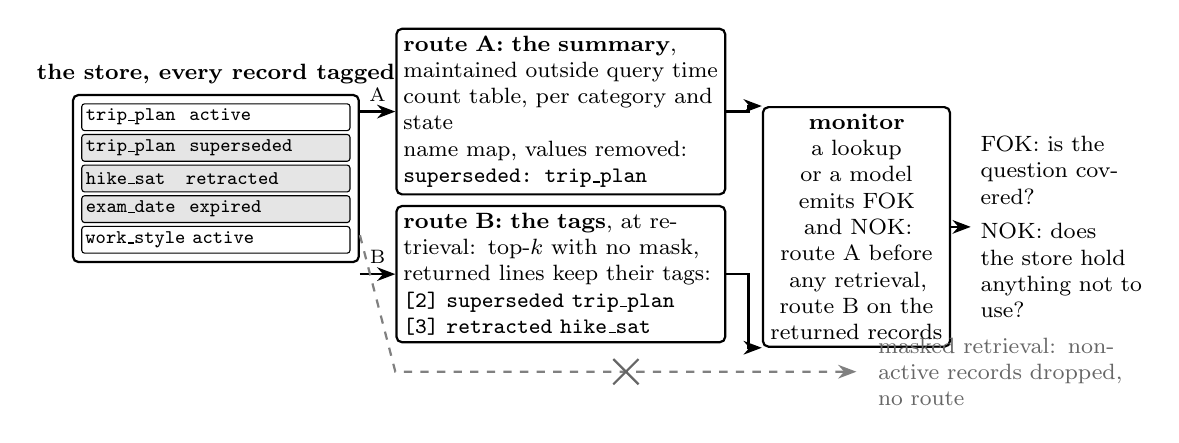
\begin{tikzpicture}[font=\footnotesize, >=Stealth,
  rec/.style={draw, rounded corners=1pt, text width=3.3cm, minimum height=0.34cm, inner sep=1.5pt, align=left, font=\scriptsize\ttfamily},
  box/.style={draw, thick, rounded corners=2pt, inner sep=2.5pt, align=left, font=\footnotesize},   % Phase 4c (L3): the drawing compacted
  route/.style={->, thick},
  grey/.style={->, thick, draw=black!50, dashed}]
  \node[rec, fill=white] (r1) {trip\_plan~~active};
  \node[rec, below=1pt of r1, fill=black!10] (r2) {trip\_plan~~superseded};
  \node[rec, below=1pt of r2, fill=black!10] (r3) {hike\_sat~~~retracted};
  \node[rec, below=1pt of r3, fill=black!10] (r4) {exam\_date~~expired};
  \node[rec, below=1pt of r4, fill=white] (r5) {work\_style~active};
  \node[draw, thick, rounded corners=2pt, fit=(r1)(r5), inner sep=3pt, label={[font=\footnotesize\bfseries]above:the store, every record tagged}] (store) {};
  \node[box, right=0.45cm of store.east, anchor=west, yshift=0.85cm, text width=4.0cm] (summ)
    {\textbf{route A: the summary}, maintained outside query time\\ count table, per category and state\\ name map, values removed:\\ \texttt{superseded: trip\_plan}};
  \node[box, below=0.12cm of summ, text width=4.0cm] (tags)
    {\textbf{route B: the tags}, at retrieval: top-$k$ with no mask, returned lines keep their tags:\\ \texttt{[2] superseded trip\_plan}\\ \texttt{[3] retracted hike\_sat}};
  \node[box, right=0.45cm of tags.east, anchor=west, yshift=0.6cm, text width=2.2cm, align=center] (mon)
    {\textbf{monitor}\\ a lookup or a model\\ emits FOK and NOK: route A before any retrieval, route B on the returned records};
  \node[right=0.25cm of mon.east, anchor=west, font=\footnotesize, align=left, text width=2.05cm] (jud) {FOK: is the question covered?\\[3pt] NOK: does the store hold anything not to use?};
  \draw[route] (store.east |- summ.west) -- (summ.west) node[midway, above, font=\scriptsize] {A};
  \draw[route] (store.east |- tags.west) -- (tags.west) node[midway, above, font=\scriptsize] {B};
  \draw[route] (summ.east) -- ++(2.8mm,0mm) |- (mon.north west);
  \draw[route] (tags.east) -- ++(2.8mm,0mm) |- (mon.south west);
  \draw[route] (mon.east) -- (jud.west);
  \coordinate (m0) at ($(store.east)+(0mm,-7.2mm)$);
  \coordinate (my) at ($(tags.south)+(0mm,-3.6mm)$);
  \coordinate (m1) at (tags.west |- my);
  \coordinate (m2) at ($(mon.south |- my)$);
  \draw[grey] (m0) -- (m1) -- (m2) node[pos=0.5, inner sep=0pt] (x) {};
  \node[right=0.15cm of m2, anchor=west, font=\footnotesize, text=black!60, align=left, text width=3.1cm] {masked retrieval: non-active records dropped, no route};
  \draw[thick, draw=black!60] ($(x)+(-1.6mm,-1.6mm)$) -- ($(x)+(1.6mm,1.6mm)$) ($(x)+(-1.6mm,1.6mm)$) -- ($(x)+(1.6mm,-1.6mm)$);
\end{tikzpicture}
\caption{The framework: a tagged store (grey rows non-active), route A (the summary, read before any retrieval) and route B (the tags on returned records, read at retrieval time) to a monitor emitting FOK and NOK; masked retrieval has no route.}
\label{fig:framework}
\end{figure}

\section{Related work}\label{sec:related}

%% Writing pass Phase 4 (2026-09-15), items 13 to 16: three paragraphs with plain topic sentences; the finding and the framing out (items 3, 14, 88);
%% the knowledge-conflict and temporal-LM work cited (item 15); STALE's citation on its name (item 16).
Metamemory studies judgments about one's own memory, and two of its judgments transfer to an external store.
Classical work treats monitoring as a judgment about memory state \citep{nelson1990,koriat1996}, and this paper asks the same two questions of a store the agent does not own.

Adaptive retrieval, abstention and calibration each decide something before or about an answer, and none has an external store to be right about.
Adaptive retrieval decides whether to query a static corpus from parametric or generated-content signals \citep{lewis2020,flare,mallen2023,ren2025,wang2023,selfrag,su2024,seakr,verbrouting,metamem}, abstention benchmarks score whether a question admits an answer \citep{rajpurkar2018,kamath2020,yang2024,abstentionbench}, and calibration work scores confidence in an answer \citep{kadavath2022,lin2022,tian2023,xiong2024}.
Those that retrieve observe a bounded view rather than a maintained summary (Section~\ref{sec:framework}).

Memory systems and memory benchmarks score what is retrieved or answered, after retrieval.
One line trains the loop that writes, updates and queries a store \citep{automem,supersede}; long-term stores \citep{packer2023,zhong2024,zhang2025survey,mem0,amem} and remembered-answer benchmarks \citep{longmemeval,locomo} measure what comes out once memory has been consulted.
Reliance on obsolete memory \citep{memora} and conflict resolution across turns \citep{memoryagentbench} are scored after retrieval too.
STALE \citep{stale}, the closest work, asks whether an agent can tell that a memory it has already retrieved is no longer valid; this paper asks whether the store holds such a memory before anything is retrieved.
Zep's validity intervals \citep{zep} are lifecycle tags of the kind route B returns.
The benchmarks that grade obligations supplied by policy or after the fact \citep{nissenbaum2004,cimemories,maini2024,gatemem,pmbench,hushbench,statemembench} grade an outcome once a cue or a revision has arrived.
Obsolete-versus-current conflict inside a store is the phenomenon that knowledge-conflict and temporal work studies inside a model \citep{xu2024conflicts,longpre2021,dhingra2022}.
What this paper measures is the judgment made before retrieval, about the store itself, from the content's own lifecycle state.

\section{Framework}\label{sec:framework}

%% Writing pass Phase 4b (2026-09-15): Section 3 written fresh from the author's skeleton (reviews/v18/tools/wp_phase4b.py). Both definitions, the grid
%% and the box are carried verbatim from the Phase 4 build; Listing 1 moves to Appendix E.3 and Figure 2 to the head of Section 5.
A store is a set of tagged records, and a question comes with an intent.
Let a store $S$ be a finite set of items $e$ with content and metadata $m(e)=(c_e,\kappa_e,\xi_e,h_e,t_e)$: category, slot key (the attribute name), lifecycle state $\xi_e\in\{\textsc{active},\textsc{superseded},\textsc{expired},\textsc{retracted}\}$, optional event-time anchor, and ingest time \citep{fr}.
The lifecycle state is the tag a record carries; expiry is a flag derived from the event-time anchor rather than a tag the store writes, so an expired record may still carry the active tag.
A record is non-active when it is superseded, retracted or expired, and a record carrying more than one mark is labelled by the first of retracted, superseded, expired (Appendix~\ref{app:glossary}).
A query $q$ has intent $i(q)\in\{\textsc{current},\textsc{upcoming},\textsc{past},\textsc{change}\}$, the time frame it asks about, because the same record can be licensed under one intent and forbidden under another.

\begin{definition}[Intent-conditional coverage]\label{def:coverage}
% C028
$\mathrm{Cov}(q,S)\in\{\present,\absent,\pn\}$.
% C029
The label is \pn{} when $S$ contains content that must be suppressed for the answer to be right under $i(q)$; \present{} denotes licensed answering content with no obligation that matters for the answer, and \absent{} denotes neither. The grid below gives the label by the state of the relevant record and the intent.
% C030: the cases of Definition 1 as the grid of Table tab:pn-grid (items 20 and 94)
\end{definition}

%% Writing pass Phase 3 (2026-09-15), items 20 and 94: Definition 1's cases as a grid (unnumbered, so the result tables keep their numbers); the CHANGE intent is never PN
%% because both the old and the new value are licensed; n.a. is a combination the definition does not assign because the question construction never produces it (Appendix E.3, where the intent is typed structurally).
\begin{center}
\scriptsize
\setlength{\tabcolsep}{5pt}
\begin{tabular}{@{}lcccc@{}}
\toprule
Relevant record & \textsc{current} & \textsc{upcoming} & \textsc{past} & \textsc{change} \\
\midrule
active, licensed & \present{} & \present{} & \present{} & \present{} \\
superseded value & \pn{} & n.a. & n.a. & \present{} \\
retracted plan & \pn{} & \pn{} & n.a. & n.a. \\
expired event & \pn{} & \pn{} & \present{} & n.a. \\
none & \absent{} & \absent{} & \absent{} & \absent{} \\
\bottomrule
\end{tabular}
\par\vspace{1pt}{\scriptsize The \textsc{change} intent is never \pn{}, because both the old and the new value are licensed; n.a.\ means a combination the question construction never produces.}
\end{center}
Both judgments are probabilities, scored by AUROC \citep{hanley1982}.
We elicit $\mathrm{FOK}(q,S)\in[0,1]$ as a probability that coverage is not \absent{} and $\mathrm{NOK}(q,S)\in[0,1]$ as a probability that coverage is \pn{}.
A blind monitor sees only the question, so its AUROC measures what the question alone gives away, and an indexed monitor also sees the store's summary.

\begin{definition}[Lifecycle summary]\label{def:index}
% C035 (R77-T1, D5); the size claim qualified to a fixed name vocabulary.
A summary $M(S)$ is maintained outside query time. Ours pairs a count table with an attribute-name map from which every stored value is removed. The count table holds each category--lifecycle count and, per category, the count of updates that superseded an entry. The name map records which names each category exposes and which carry superseded content; the names that carry superseded content form the superseded-names list. The size $|M(S)|$ is $O(|C|\cdot|\Xi|+|N|)$ in the number $N$ of distinct names exposed, and for a fixed name vocabulary it is independent of the number of records $|S|$.
\end{definition}
A rendered summary is Listing~\ref{lst:summary} in Appendix~\ref{app:construction}; the count table is included because it was part of the summary as fixed before the study.
%% Writing pass Phase 3 (2026-09-15), item 17 with its addendum and item 23: the notation box directly after Definition 2, twelve rows; every term is used verbatim
%% from here on (ground rule 3). The vocabulary of names / counts / reads leaves the prose of Section 3 for the box (its E.1 copy stands until item 69).
\begin{center}
\setlength{\fboxsep}{1.5pt}%% Phase 4c (L4): the frame and row spacing tightened; the words are unchanged
\fbox{\begin{minipage}{0.97\linewidth}
\scriptsize
\setlength{\tabcolsep}{1.5pt}
\renewcommand{\arraystretch}{0.92}
\noindent\textbf{Notation.} The terms below are used verbatim throughout.\par
\noindent\begin{tabular}[t]{@{}p{0.115\linewidth}p{0.36\linewidth}@{}}
\midrule
lifecycle state; non-active & the tag a record carries, \textsc{active}, \textsc{superseded}, \textsc{retracted} or \textsc{expired}; the last three are the non-active states \\
forbidding record & the non-active record that would make an answer wrong if used \\
intent; \pn{} & the time frame a question asks about (\textsc{current}, \textsc{upcoming}, \textsc{past}, \textsc{change}); present-negative: the store holds relevant content and using it would make the answer wrong. An \emph{obligation} is a question whose label is \pn{} \\
FOK; NOK & the coverage judgment, is the question covered; the obligation judgment, does the store hold anything not to use \\
summary & the count table (records per category and lifecycle state) and the name map (the attribute names each category exposes, values removed); the superseded-names list is the part of the name map that carries superseded content \\
named state; counted state & a state whose attribute names the summary lists (superseded, by default); a state the summary only counts (retracted, expired) \\
\end{tabular}\hfill\begin{tabular}[t]{@{}p{0.115\linewidth}p{0.36\linewidth}@{}}
\midrule
names, counts, reads & a summary \emph{names} a state when it lists the attribute names in that state and \emph{counts} it when it gives only a count of it; a reader \emph{reads} a state when its score separates that state's items from the rest \\
blind; indexed & the monitor sees the question alone; the monitor sees the question and the summary \\
gain ($\Delta$) & the indexed score minus the blind score on the same questions; on the counterfactual set the blind score is $0.50$ by construction, so there the AUROC and the gain carry the same information \\
ground-truth summary; store-written summary & the summary built from ground truth; the summary built from the fields the backend itself exposes \\
name lookup; all-states lookup & the similarity lookup over the summary's superseded-names list, the no-model baseline every model is measured against; the same over a list that names all three non-active states \\
route A; route B & the summary route, read before any retrieval; the tag route, retrieval without a mask whose returned records keep their tags, read at retrieval time (Figure~\ref{fig:framework}) \\
\end{tabular}
\end{minipage}}
\end{center}

%% The skeleton's third paragraph: the mask claim and Figure 1's no route. Item 19's sentence is gone; the two-store argument ("ranks below $k$ common items")
%% is Phase 5's appendix item; item 14's framing sentence ("the summary route is retrieval over a metadata index") is dropped under the skeleton, reported.
A retriever that masks non-active records from its ranking, as lifecycle-tracking and overwriting stores do, cannot supply the obligation judgment on its own, because the mask drops the records whose tags carry it.
That is the crossed-out path of Figure~\ref{fig:framework}, masked retrieval with no route.

\section{Setup}\label{sec:setup}

%% Writing pass Phase 4b (2026-09-15): Section 4 written fresh from the author's skeleton (reviews/v18/tools/wp_phase4b.py). Table 1 is carried with its
%% note reduced to the draws; Figure 2's source moves to the head of Section 5. The 5% mask pass rate (Appendix E.9), the 5.2% presence bound (E.3),
%% the 0.80 to 0.97 question probes (Appendix C) and the 58 / 16 predictions (Appendix F) are kept with their pointers.
Of the three backends, FR-Bank \citep{fr} is the only one that tags every entry with a lifecycle state.
Its stock configuration masks non-active records from retrieval, and under that mask its own retraction questions pass at $5\%$ (Appendix~\ref{app:census}).
Mem0 (\texttt{mem0ai} 1.0.5) overwrites the record it exposes and A-MEM links notes \citep{mem0,amem}; neither records lifecycle structure, so we call them the structureless backends.
The models are OpenAI's GPT-4.1 mini, GPT-5.6 Luna and GPT-5.6 Sol, Anthropic's Haiku 4.5 and Opus 5, and Moonshot's Kimi K3 with open weights.
GPT-4.1 mini ran the main study at one call per question, Opus 5, Haiku 4.5 and GPT-5.6 Luna ran every population at five calls, and GPT-5.6 Sol and Kimi K3 ran the cross-model set only (Table~\ref{tab:setup}).

Every question set was generated with large language models from human-written manifests of synthetic users (personas), and the manifests are the ground truth every label is scored against.
Labels follow Definition~\ref{def:coverage}; the intent is fixed by the question's construction and used only to label, the monitor is never told it, and every \pn{} label was verified by hand.
A presence control confirms that each target is stored, so the chance that an \absent{} label is wrong is $5.2\%$ at the observed base rate (Appendix~\ref{app:construction}).
Table~\ref{tab:setup} (Appendix~\ref{app:laddertable}) names every population with its size, positives and models, and every later number is stated on one of them.
Appendix~\ref{app:provenance} traces each headline number to its labels, tag source and evaluator.


A ground-truth summary is built from ground truth and a store-written summary from the fields the backend itself exposes, rendered by the same code with a cap of fifteen names per list.
%% R112 (2026-09-15), review-2 A1 (the author's ruling): the term defined once; on Mem0 and A-MEM the TRUE index is the manifest rendered
%% under the backend's constraints (e1_metamemory/indexes_v2.json meta.availability). reviews/v19/A1_CONSTRAINED_RENDERING.md.
%% Page ruling (2026-09-15): one sentence of at most 28 words (18, one line); the full form (no categories or names; exact totals, every name section not expressible) is E.7's.
On Mem0 and A-MEM it is the manifest rendered under the backend's constraints, the constrained rendering (Appendix~\ref{app:inversion}).
%% R110: the cap and its recorded reason; the sixty-percent line's provenance (A5_EDITS.md item 9; AUX-E1R-NB6 1.75; indexes_s2u.json meta 15.04).
The cap, fixed before the pilot, never binds on the ground-truth summary, whose superseded list averages under two names; it binds on the store's own metadata, reported capped and with the cap lifted (Appendix~\ref{app:repro}).

The monitor returns a probability under a fixed rubric, and the blind and the indexed prompt differ only in whether the summary precedes the question, so the gain isolates the summary (Appendix~\ref{app:construction}).
The name lookup, the baseline every model is measured against, scores each question by its maximum cosine similarity under the sentence encoder \texttt{all-MiniLM-L6-v2} to the summary's superseded-names list (Appendix~\ref{app:baselines}).
We report the item-level paired bootstrap interval first and the persona-grouped interval second, and where they disagree the wider decides.
We call a difference \emph{reliable} when both intervals exclude zero, and \emph{within tolerance} when $|\Delta| \le 0.05$.
On the counterfactual set the persona-grouped interval is the one printed, because resampling whole questions keeps each triple intact.
Question wording alone carries much of a blind score: probes on the question text reach $0.80$ to $0.97$ (Appendix~\ref{app:questionprior}), which is why we report paired gains and the counterfactual set.
Of the $58$ predictions preregistered before data collection, $16$ came out otherwise (Appendix~\ref{app:registration}).

\section{The clean test: one question, three stores}\label{sec:counterfactual}

\begin{figure}[t]
\centering
%% Writing pass Phase 4b (2026-09-15): Figure 2's source at the head of Section 5, the section that reads the triples (the author's option).
%% R110: Figure 2, the worked example (CC_PASS_v18 section 3.4): two real triples of the counterfactual set (r82_counterfactual/cf2/cf_cell.json,
%% cf_indexes.json v2 texts): cf2:alex:work_preference (supersession) and cf2:bruna:trip_plan:brazil_carnival (retraction); the summary lines
%% that differ across the three versions, transcribed; the lookup's score under each version (reviews/NUMBERS_R110.md AUX-R110-FIG2). Labels \footnotesize (8 pt).
\footnotesize
\setlength{\tabcolsep}{2pt}
\renewcommand{\arraystretch}{0.95}
%% Phase 4c (L1): the row padding tightened and the outer columns widened so no cell wraps; the words are unchanged.
\begin{tabular}{@{}>{\raggedright\arraybackslash}p{0.34\linewidth}>{\raggedright\arraybackslash}p{0.20\linewidth}>{\raggedright\arraybackslash}p{0.20\linewidth}>{\raggedright\arraybackslash}p{0.23\linewidth}@{}}
\multicolumn{4}{@{}l}{\textbf{A retraction triple.} Question: \textit{What should I expect during my next Brazil Carnival trip?}}\\
\toprule
summary line & version 1: \present{} & version 2: \pn{} & version 3: \absent{}\\
\midrule
lifecycle total, retracted & \texttt{0} & \texttt{1} & \texttt{0}\\
\texttt{PROJECTS\_ENDEAVORS}: entries, active, retracted & \texttt{55, 55, 0} & \texttt{56, 55, 1} & \texttt{54, 54, 0}\\
names in the category & \texttt{..., trip\_plan} & \texttt{..., trip\_plan} & \texttt{...} (no \texttt{trip\_plan})\\
names carrying superseded content & \texttt{(none)} & \texttt{(none)} & \texttt{(none)}\\
the name lookup's score & $0.00$ & $0.00$ & $0.00$\\
the label & the trip is on & the trip was cancelled & no such record\\
\bottomrule
\end{tabular}
\caption{A retraction triple of the counterfactual set: one question, three store versions differing in one attribute; only the differing summary lines are shown, with the name lookup's score. Only the count row differs, so no reader over names separates the versions (supersession triple: Appendix~\ref{app:counterfactual}).}
\label{fig:example}
\end{figure}

When the question is fixed and only the store changes, the models' judgment tracks the attribute names in the summary; the count interventions do not establish that it tracks the counts.
The counterfactual set asks $148$ questions of three versions of one store that differ in one attribute.
The questions were written before any version of the store existed, so the same wording gets three labels and the summary is the only input that varies.
Blind NOK is $0.50$ by construction on this set, so each gain below is the AUROC minus that chance value.
Table~\ref{tab:cf-main} gives every reader on the whole set and Figure~\ref{fig:perstate} per state, with two readers that have no model in them.
One is the name lookup, a similarity lookup over the superseded-names list; the other is a count reader that guesses the question's category from its text and reads that category's retracted and expired \emph{counts}.
A category-aware count reader, which takes the category from the manifest, is that reader's upper bound on the two counted states.

\begin{table}[h]
%% Writing pass Phase 1 (2026-09-15), item 50 with its addendum: two decimals; one quantity per column, the profile-grouped interval of the AUROC on every row
%% (the model rows' AUX-CF2-*-V2 / -V3 'indexed persona-clustered' intervals, the gain interval shifted by the blind 0.5000; no item-level AUROC interval is recorded,
%% so the item-level intervals of the gain stay in Appendix C.2, tab:counterfactual); the count readers AUX-R110-A1-CR; the readers with no model under a rule.
%% The per-state columns stay until the per-state figure of item 30 lands (Phase 3). 0.92 lives in this table and in C.2 only (P4).
\caption{Obligation AUROC on the counterfactual set ($n=444$; positives $88$ supersession, $30$ retraction, $30$ expiry), whole set, with the persona-grouped interval of the AUROC; the per-state values are Figure~\ref{fig:perstate}. Blind NOK is $0.50$ by construction, so the gain is the AUROC minus $0.50$. PN vs PRESENT and W/T/L are post hoc (Appendix~\ref{app:counterfactual}); the item-level paired gain intervals are there too.}
\label{tab:cf-main}
\centering
\scriptsize
\setlength{\tabcolsep}{3pt}
%% R112 (2026-09-16), post hoc: the PN vs PRESENT column and the W/T/L column from reviews/NUMBERS_WP.md section 8 (AUX-WP-B-PNPRESENT, -B-ORDERING; two-decimal forms ledgered there).
\begin{tabular}{@{}lrlrl@{}}
\toprule
Reader, summary & AUROC & persona interval & PN vs PRESENT & W/T/L \\
\midrule
GPT-4.1 mini, sup.\ only & $0.72$ & $[0.67,0.76]$ & $0.71$ & $81/57/10$ \\
GPT-4.1 mini, all three & $0.80$ & $[0.74,0.85]$ & $0.78$ & $105/32/11$ \\
Haiku 4.5, sup.\ only & $0.76$ & $[0.71,0.80]$ & $0.75$ & $89/52/7$ \\
Haiku 4.5, all three & $0.88$ & $[0.84,0.91]$ & $0.87$ & $125/18/5$ \\
Opus 5, sup.\ only & $0.84$ & $[0.80,0.88]$ & $0.84$ & $128/3/17$ \\
Opus 5, all three & $0.91$ & $[0.88,0.94]$ & $0.91$ & $139/0/9$ \\
\midrule
\multicolumn{5}{@{}l}{\textit{Readers with no model in them}}\\
Name lookup, sup.\ only & $0.77$ & $[0.72,0.81]$ & $0.77$ & $82/66/0$ \\
All-states lookup, all three & $0.88$ & $[0.84,0.91]$ & $0.87$ & $121/27/0$ \\
Category-guessing count reader, sup.\ only & $0.66$ & $[0.63,0.70]$ & $0.64$ & $65/83/0$ \\
Category-aware count reader, sup.\ only & $0.60$ & $[0.58,0.64]$ & $0.59$ & $60/88/0$ \\
\bottomrule
\end{tabular}
\end{table}

\begin{figure}[t]
\centering
%% Writing pass Phase 3 (2026-09-15), item 30 with its addendum: per-state AUROC on the counterfactual set as two panels sharing the y-axis (left the superseded-only
%% summary, right the all-states summary), four states, one bar per reader within each state, a dashed line at 0.50, y from 0.4 to 1.0; the count reader has no
%% all-states variant. Values as in Table tab:cf-main and Appendix C.2 (AUX-CF2-NB6-V2, -ALLSTATES-V3, -MINI/-H45/-OP5-V2/-V3, AUX-CF2-PERSTATE, AUX-R110-A1-CR).
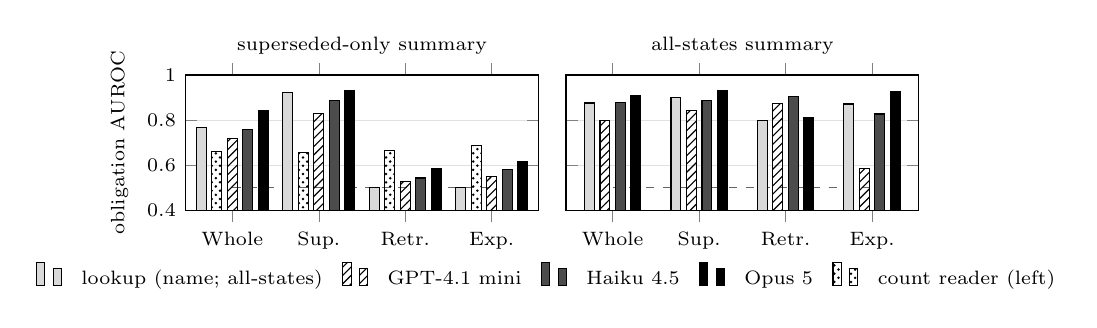
\begin{tikzpicture}
\begin{groupplot}[group style={group size=2 by 1, horizontal sep=0.35cm, ylabels at=edge left, yticklabels at=edge left},
    ybar, /pgf/bar width=3.6pt, width=0.5\linewidth, height=3.3cm, ymin=0.4, ymax=1.0,
    ylabel={obligation AUROC}, ylabel style={font=\scriptsize}, symbolic x coords={Whole,Sup.,Retr.,Exp.}, xtick=data, enlarge x limits=0.18,
    tick label style={font=\scriptsize}, title style={font=\scriptsize, yshift=-2pt}, ymajorgrids, grid style={black!12},
    legend style={at={(-0.05,-0.34)}, anchor=north, legend columns=5, font=\scriptsize, draw=none, fill=none, column sep=5pt}]
  \nextgroupplot[title={superseded-only summary}]
      \draw[dashed, black!60] (axis cs:Whole,0.5) -- (axis cs:Exp.,0.5);
      \addplot[draw=black, fill=black!15] coordinates {(Whole,0.7663) (Sup.,0.9223) (Retr.,0.5000) (Exp.,0.5000)};
      \addplot[draw=black, fill=black!45, pattern=crosshatch dots, pattern color=black] coordinates {(Whole,0.6623) (Sup.,0.6573) (Retr.,0.6669) (Exp.,0.6872)};
      \addplot[draw=black, fill=white, pattern=north east lines, pattern color=black] coordinates {(Whole,0.7167) (Sup.,0.8308) (Retr.,0.5283) (Exp.,0.5489)};
      \addplot[draw=black, fill=black!70] coordinates {(Whole,0.7566) (Sup.,0.8876) (Retr.,0.5433) (Exp.,0.5794)};
      \addplot[draw=black, fill=black] coordinates {(Whole,0.8405) (Sup.,0.9325) (Retr.,0.5872) (Exp.,0.6150)};
  \nextgroupplot[title={all-states summary}]
      \draw[dashed, black!60] (axis cs:Whole,0.5) -- (axis cs:Exp.,0.5);
      \addplot[draw=black, fill=black!15] coordinates {(Whole,0.8756) (Sup.,0.8995) (Retr.,0.7975) (Exp.,0.8711)};
      \addplot[draw=black, fill=white, pattern=north east lines, pattern color=black] coordinates {(Whole,0.7967) (Sup.,0.8444) (Retr.,0.8725) (Exp.,0.5869)};
      \addplot[draw=black, fill=black!70] coordinates {(Whole,0.8773) (Sup.,0.8852) (Retr.,0.9042) (Exp.,0.8269)};
      \addplot[draw=black, fill=black] coordinates {(Whole,0.9079) (Sup.,0.9319) (Retr.,0.8100) (Exp.,0.9267)};
      \addlegendimage{draw=black, fill=black!45, pattern=crosshatch dots, pattern color=black}
      \legend{lookup (name; all-states), GPT-4.1 mini, Haiku 4.5, Opus 5, count reader (left)}
\end{groupplot}
\end{tikzpicture}
\caption{Obligation AUROC on the counterfactual set per state, under the superseded-only summary (left) and the all-states summary (right); the dashed line is chance. On the state the summary names the lookup and the models are high together; on the states it only counts, every model discriminates more weakly than the count reader, and naming those states lifts every reader.}
\label{fig:perstate}
\end{figure}

%% The author's paragraph of 2026-09-15 (the ruling on the Phase 1 report; items 31 and 33), one number per sentence; its third sentence ("Most questions name the attribute they ask about (111 of the 204 drafted)") is held back:
%% AUX-CF2-QUESTIONREAD's 111 of 204 counts questions that name a specific value beyond their topic (the G.2 flag), not questions that name their attribute. AUX-E1R-NB6 (1.75); AUX-R104-MARGIN (+0.0742).
Supersession is the one state the summary \emph{names}.
The superseded-names list averages $1.75$ names on the full obligation set.
The lookup therefore has the target's name in front of it, and the question is what a model adds.
On the counterfactual set, GPT-4.1 mini and Haiku 4.5 do not exceed the name lookup and Opus 5 exceeds it by $0.07$ (Table~\ref{tab:cf-main}).
%% R112 (2026-09-16), post hoc B1-B3 (reviews/NUMBERS_WP.md section 8): the largest move from the pooled AUROC is 0.0230; the coverage-only reference is 0.75 pooled and ties every triple.
Scored against the PRESENT versions alone, which also hold relevant content, every reader moves by at most $0.03$ from its whole-set value, so the comparison stands where coverage is equal.
Table~\ref{tab:cf-main} gives that score and the wins, ties and losses per triple, both post hoc.
A reader that only knows whether the store covers the question would score $0.75$ on the whole set and tie every triple.

%% Writing pass Phase 1 (2026-09-15), items 87 and 90: the own-name ablation paragraph from Section 6, in three sentences (AUX-RESP-L1-MINI: 0.8572 to 0.5310, -0.3262; AUX-RESP-A1-H45-OWN: 0.8897 to 0.6759, -0.2139; whole 0.6882).
The summary route rests on names, because removing them removes the judgment.
Taking the target's own name and its nearest neighbours out of the superseded-names list drops GPT-4.1 mini's supersession judgment from $0.86$ to $0.53$ on the full obligation set ($63$ supersession obligations), a reliable drop.
The same edit drops Haiku 4.5's reliably from $0.89$ to $0.68$, while Haiku 4.5 keeps $0.69$ on the whole population (Appendix~\ref{app:resp}).

%% R110: the count-reader paragraph (READER_CLAIM.md section 2, the author's rulings of 2026-09-14 and 2026-09-15; AUX-R110-A1-CR, -MODELS, -V2R; AUX-CF2-EQUIV-V2R; AUX-V2RCAT-MINI, -H45, -REF).
The retracted and expired states are recoverable from the count table, and every tested model separates them more weakly than a count reader does.
The category-guessing count reader separates the retracted versions at $0.67$ and the expired at $0.69$ ($30$ pairs each), its category-aware oracle at $0.73$ and $0.78$, where every model scores $0.53$ to $0.62$.
% AUX-R110-A1-CR: the category-guessing reader 0.6669 / 0.6872, the category-aware reader 0.7306 / 0.7778 on retraction / expiry (Table tab:cf-cr); the models 0.5283 to 0.6150 (reviews/NUMBERS_WP.md section 5)
In most retraction pairs and half the expiry pairs the category has no other such entry ($26$ of $30$ and $15$ of $30$), so the count goes from zero to one.
Permuting the lifecycle totals across the store versions moves no tested model by more than $0.01$.
%% R112 (2026-09-16), review-2 item E (the author's form, one interval in prose under Q-B): AUX-V2RCAT-MINI expiry +0.0611 [-0.0404, +0.1641] / [-0.0217, +0.1417]; Haiku 4.5 -0.0072 / -0.0453; Opus 5 not run.
Moving the obligation's own increment to a sibling version, the moved-count control, sends a count reader below chance.
GPT-4.1 mini moves $+0.06$ on expiry with interval $[-0.04,+0.16]$ and Haiku 4.5 stays within tolerance (Appendix~\ref{app:counterfactual}); Opus 5 was not run on this control.
Under the tested prompts the names carry the judgment, and the count representations tested carry no signal we can detect.

A count cannot say which attribute is retracted or expired.
When the summary names those attributes, every model improves (Table~\ref{tab:cf-main}).
Every model then separates the retracted versions, and all but GPT-4.1 mini the expired ones (Figure~\ref{fig:perstate}).
The all-states lookup scores $0.88$ on the whole set, and Haiku 4.5 gains a reliable $+0.30$ on the two counted states once they are named.
% AUX-CF2-ALLSTATES-V3 (0.8756); AUX-CF2-COUNTED (Haiku +0.30); AUX-CF2-OP5-V3 (0.9079, +0.0323)
The counted-state evidence rests on $30$ retraction and $44$ expiry pairs, the $30$ plus the $14$ of the descriptive extension draw in Appendix~\ref{app:counterfactual}.
On the full obligation set the counted-state groups are $26$ retraction and $15$ expiry obligations, and their rows give only a direction (Section~\ref{sec:populations}).

%% Writing pass Phase 1 (2026-09-15), item 90: the list-length paragraph to two sentences; the padding curve (AUX-PAD-*, Table tab:pad), the store's own pool (AUX-R110-A4, moved to C.2) and the contamination figures (AUX-PAD-C-*) stand in Appendix C.2.
The lookup works because the list is short and clean; as it grows or fills with wrong names, the lookup and the models fall together (Appendix~\ref{app:counterfactual}).

\section{Two routes to the obligation}\label{sec:routes}

A retriever that returns non-active records with their tags is a second route to the obligation, read at retrieval time from the returned records (route B in Figure~\ref{fig:framework}).
It covers the states the list does not name.
A five-record view holds the forbidding record for $54$ of the $104$ obligations on the full obligation set, a reach of $0.52$.
Shown that view and no summary, GPT-4.1 mini scores $0.69$ against $0.73$ under the summary; shown both, $0.83$ (Table~\ref{tab:routes}, Appendix~\ref{app:resp}).
The retriever is FR-Bank's own cosine search with its mask off, each line carrying the ground-truth tag (Appendix~\ref{app:resp}).
% AUX-R104-REACH


Per state the two routes are mirror images.
On the full obligation set the tagged view leads the summary on expiry by a reliable $+0.24$ and trails it on supersession by a reliable $-0.17$.
The reason is that a retrieved entry tagged retracted or expired is a name the summary never lists (Appendix~\ref{app:resp}).
Shown both, GPT-4.1 mini gains a reliable $+0.10$ over the summary alone.
Haiku 4.5 scores $0.79$ shown both against $0.82$ under its summary alone, so the combined monitor is best for GPT-4.1 mini only (Appendix~\ref{app:resp}).
% AUX-RESP-RETRIEVED, AUX-RESP-HYBRID, AUX-RESP-A1-H45-HYBRID (0.7863), -H45-RETRIEVED (0.7134)

%% R110: the own-marks paragraph per A2 branch B3 and the reach follow-up (AUX-R110-A2, -OWNVSJOIN, -REACH; AUX-RESP-A1-BELIEVED; lock_amend1.json).
With the store's own tags instead of ground-truth tags, the same view scores higher.
FR-Bank's tags mark $1{,}389$ of the $3{,}305$ lines shown as non-active where the ground-truth tags mark $217$, a precision of $0.14$.
GPT-4.1 mini's obligation score on that view rises from $0.69$ to a reliable $0.81$.
The reason is reach rather than volume.
The store's tags mark $70$ of the $99$ forbidding records in view against the ground-truth tags' $60$, while a count of tagged lines scores $0.62$ under either tag source (Table~\ref{tab:routes-full}, Appendix~\ref{app:resp}).
% AUX-R110-A2 (TD 0.6157 / 0.6209; TL 0.6523); AUX-R110-A2-OWNVSJOIN (FR 0.6683 / 0.7212; 70 / 60 / 99); +0.0932


\section{What backends write about themselves}\label{sec:backends}\label{sec:inversion}\label{sec:stores}

No tested backend writes the list: FR-Bank over-marks, Mem0 overwrites, and A-MEM's links dangle (Table~\ref{tab:census}).
FR-Bank marks $5{,}968$ of its $18{,}936$ entries inactive where the manifest explains about $102$, and still lists $40$ of the $104$ entries the manifest's supersessions touch as active.
% AUX-SIDE-S2-CENSUS (5,968 / 102 = 58.5; 40 of 104)
Mem0 erases at its retrieval surface: of its $10{,}074$ entries, $12.7\%$ expose \texttt{updated\_at} and nothing else, because an \texttt{UPDATE} replaces the record that \texttt{search} and \texttt{get\_all} return (\texttt{mem0ai} 1.0.5).
A-MEM invents: all $23{,}186$ link references across its $11{,}319$ notes resolve to zero note identifiers (Table~\ref{tab:census}).
%% R112 (2026-09-16): the forty-persona Graphiti census (r85_graphiti/NUMBERS_R85.md AUX-R85-G10-CENSUS-FORBIDDING-FULL 13 / 34 = 0.3824 on the FULL-variant obligations, the main-text reading under D-R85-16; precision 54 / 807 = 0.0669; the registered 30 / 74 and P1's text in Appendix G.4).
On Graphiti \citep{zep}, a fourth backend whose validity intervals are the closest thing to lifecycle tags in a shipped store, a census over forty personas recovers some of the forbidding records.
Its invalidation marks reach $13$ of the $34$ obligations of the full store that the ground truth marks superseded or expired, more than the quarter we had predicted.
Of its $807$ non-active edges, $54$ fall on such a record (Appendix~\ref{app:posthoc-graphiti}).

\begin{table}[h]
%% Writing pass Phase 1 (2026-09-15), items 52 and 90: three rows, one sentence per cell; the Conflate row's content is in Appendix E.9 as prose. AUX-SIDE-S2-CENSUS, AUX-BELIEVED-MEM0, the R86 census (A-MEM).
\caption{A census of what each backend writes about itself, scored against the ground-truth manifests: counts with no sampling interval. FR-Bank's conflation of retraction with supersession is described in Appendix~\ref{app:census}.}
\label{tab:census}\censusalias%% R112 (2026-09-16): the alias label for the frozen DS paragraph's reference in Appendix E.10 (review-2 F6)
\centering
\scriptsize
\setlength{\tabcolsep}{2pt}
\begin{tabular}{@{}p{0.12\linewidth}p{0.10\linewidth}p{0.70\linewidth}@{}}
\toprule
Backend & Mode & Census measurement \\
\midrule
FR-Bank & Overstate & Of $18{,}936$ entries and $109$ events, marks $5{,}968$ entries stale against ${\sim}102$ in ground truth (about $58\times$) and retains an active obsolete assertion after $72\%$ of supersession events, at the stored-versus-obsolete matching threshold of the census. \\
Mem0 & Erase & Of $10{,}074$ entries, $12.7\%$ expose \texttt{updated\_at} and nothing else, because \texttt{UPDATE} overwrites the record it exposes (version 1.0.5) and ingestion is silently lossy. \\
A-MEM & Invent & All $23{,}186$ link references across $11{,}319$ notes resolve to $0$ note identifiers, on the $40$ scored personas. \\
\bottomrule
\end{tabular}
\end{table}


FR-Bank's own metadata leaves GPT-4.1 mini and the name lookup close to chance and costs Haiku 4.5 about a quarter of its gain.
The store-written summary is read capped (with the renderer's fifteen-name cap in place) and lifted (with the cap removed).
On the full obligation set GPT-4.1 mini and the lookup score $0.60$ and $0.59$ capped and $0.65$ and $0.66$ lifted, while Haiku 4.5 scores $0.71$ capped and $0.74$ lifted.
Haiku 4.5 keeps $72\%$ of its gain capped and $79\%$ lifted (Table~\ref{tab:levels}, Appendix~\ref{app:census}).
% AUX-E1R-BELIEVED-NOK, AUX-SIDE-S2-MINI, AUX-E1R-NB6, AUX-BH-LOOKUP-LIFTED, AUX-BH-H45-15 / -LIFTED, AUX-BH-RETENTION-15 / -LIFTED

%% Writing pass Phase 1 (2026-09-15), item 90: the own-name split in four sentences (AUX-BH-SPLIT: 0.8658 / 0.8855 on 53; 0.6839 on 10; lookup 0.7593 / 0.7969 [0.6722, 0.8992]; AUX-RESP-A1-H45-OWN 0.6882);
%% the capped halves (24 / 39; 0.6933; lookup 0.7292 / 0.6146), Haiku minus the lookup (+0.1065) and the contamination sentences (AUX-PAD-C-*) stand in Table tab:bh-split and Appendix C.2.
Where the store still writes the item's own name, Haiku 4.5 scores as it does under the ground-truth summary; where the name is gone it falls to the level the own-name ablation produced (Section~\ref{sec:counterfactual}).
On the $53$ of the $63$ supersession obligations whose name survives under the lifted rendering, Haiku 4.5 scores $0.87$ against $0.89$ under the ground-truth summary, and $0.68$ on the $10$ whose name is gone. The lookup on the same halves is in Table~\ref{tab:bh-split} (Appendix~\ref{app:census}).

%% Writing pass Phase 1 (2026-09-15), item 1: the structureless-store paragraph cut; the compression reading and the U1 disclosure stand verbatim in Appendix E.7 (pinned once).
%% R112 (2026-09-15), review-2 A1 (the author's ruling): the loss is on the constrained rendering; the store-written sentence's phrasing from
%% AUX-WP-A1-BELIEVED-BLIND (reviews/NUMBERS_WP.md section 6: Mem0 -0.0005, A-MEM -0.0313, both intervals include zero, |delta| <= 0.05).
%% Page ruling (2026-09-15): the 'at every scale' sentence cut; the pooled-66 ladder stands in E.7 with its own pointer.
The constrained rendering loses coverage on both structureless stores.
Under it GPT-4.1 mini loses $0.10$ on Mem0 and $0.11$ on A-MEM, and on the pooled $66$ questions of both stores GPT-5.6 Luna loses $0.34$ and GPT-5.6 Sol $0.10$, every interval excluding zero.
The summaries the stores themselves write are within tolerance of blind, $0.57$ against $0.57$ on Mem0 and $0.53$ against $0.56$ on A-MEM (Appendix~\ref{app:inversion}).
A name-bearing summary rebuilt from ground truth restores coverage to $0.90$ on A-MEM and $0.88$ on Mem0, so what the constrained rendering loses is the names.
The loss is compression of the indexed score toward one low value, and what triggers it is unresolved (Appendix~\ref{app:inversion}).

\section{Replication across models and the coverage judgment}\label{sec:populations}\label{sec:calibration}\label{sec:coverage}\label{sec:discrimination}\label{sec:calibration-secondary}\label{sec:ladder}

%% Writing pass Phase 1 (2026-09-15), item 2: the old Section 8 split; this section keeps the replication and the coverage result.
The obligation gain replicates across six models from three vendors.
Every paired gain excludes zero where the blind score varies, on the cross-model set (Table~\ref{tab:ladder-exact}, Appendix~\ref{app:laddertable}) and on the full obligation set (Table~\ref{tab:e1}).
On the cross-model set the five models with a varying blind score gain $+0.15$ to $+0.45$, Kimi K3 among them at $+0.26$.


\begin{table}[h]
%% Writing pass Phase 1 (2026-09-15), item 54: two ruled panels (FOK by backend; NOK by model), 'Indexed (ground-truth summary)', two decimals. Values as in v18 (AUX-E1R-*; AUX-R74-X4-*).
\caption{Blind and indexed judgments with the paired gain and both intervals: coverage by backend for GPT-4.1 mini (positives non-\absent{}) and the obligation judgment on FR-Bank by model (positives \pn{}). On the hard tier every coverage positive is an obligation, so that FOK row scores the same positives as the NOK row.}
\label{tab:e1}
\centering
\scriptsize
\setlength{\tabcolsep}{2pt}
\renewcommand{\arraystretch}{0.9}%% Phase 4c ruling: row padding 0.9; the values are unchanged
\begin{tabular}{@{}lrrrrll@{}}
\toprule
\multicolumn{7}{@{}l}{\textbf{FOK by backend, GPT-4.1 mini}}\\
Backend & $n$ / pos. & Blind & \hd{Indexed}{(ground-truth; constrained on Mem0, A-MEM)} & $\Delta$ & item interval & persona interval \\
\midrule
FR-Bank hard tier & $307$ / $35$ & $0.50$ & $0.70$ & $+0.20$ & $[+0.09,+0.32]$ & $[+0.13,+0.28]$ \\
Mem0 & $238$ / $94$ & $0.57$ & $0.48$ & $-0.10$ & $[-0.17,-0.03]$ & $[-0.16,-0.03]$ \\
A-MEM & $284$ / $126$ & $0.56$ & $0.45$ & $-0.11$ & $[-0.17,-0.04]$ & $[-0.17,-0.04]$ \\
\midrule
\multicolumn{7}{@{}l}{\textbf{NOK by model, FR-Bank}; the name lookup scores $0.75$ on the same $661$ questions}\\
Model & $n$ / pos. & Blind & \hd{Indexed}{(ground-truth summary)} & $\Delta$ & item interval & persona interval \\
\midrule
Haiku 4.5 & $661$ / $104$ & $0.42$ & $0.82$ & $+0.41$ & $[+0.33,+0.48]$ & $[+0.31,+0.50]$ \\
Opus 5 & $661$ / $104$ & $0.64$ & $0.83$ & $+0.19$ & $[+0.14,+0.24]$ & $[+0.12,+0.25]$ \\
GPT-5.6 Luna & $661$ / $104$ & $0.45$ & $0.82$ & $+0.37$ & $[+0.29,+0.44]$ & $[+0.27,+0.47]$ \\
\bottomrule
\end{tabular}
\end{table}

The coverage margin over the name lookup does not survive a lookup over the whole name map.
On the easy tier ($354$ questions), where the positives are ordinary present records, GPT-4.1 mini scores $0.78$ against the name lookup's $0.61$, a reliable margin.
%% R112 (2026-09-16), post hoc F1 (reviews/NUMBERS_WP.md section 10, AUX-WP-F1-WHOLEMAP): whole-map lookup 0.7469; model minus whole-map +0.0367 [-0.0127, +0.0861] / [-0.0036, +0.0776].
A lookup over every name in the map, computed post hoc, scores $0.75$ on the same questions, and the model's margin over it is $+0.04$ with interval $[-0.01,+0.09]$, which is not a reliable one (Appendix~\ref{app:baselines}).
On the hard tier every coverage positive is an obligation, so the coverage and obligation scores are one row, and the lookup's $0.79$ against the model's $0.70$ is not a reliable difference.
FOK detects a missing topic and not a single deleted record, which is NOK's target (Appendix~\ref{app:construction}).
The score ranks well and calibrates badly (Appendix~\ref{app:posthoc}), so a deployed monitor thresholds at the base rate of positives.

\section{Acting on the judgment}\label{sec:downstream}

%% Writing pass Phase 1 (2026-09-15), item 2: the downstream experiment split out of the old Section 8 as Section 9; the opener from the old section's first paragraph.
Acting on the judgment changes the answer stage one link at a time.
The links are reach, the tags, the store's untagged duplicates and their repair.

\begin{table}[h]
%% Writing pass Phase 1 (2026-09-15), item 55: self-explanatory headers, the 0.80-threshold note below the table, two decimals; values as in v18 (AUX-DS-AUDIT-RATES: 8/42, 8/62, 6/58, 13/82, 16/85; AUX-DS-A7-REPORTED 11/65; AUX-R104-REACH; AUX-DS-A4-*).
\caption{The downstream policies for GPT-4.1 mini on the full obligation set: forbidding records put in view, detector-flagged stale answers at the $0.50$ threshold, and correct answers on the licensed items. The flagged rate holds under every gated policy until the store's untagged duplicates are retagged (Table~\ref{tab:ds-a5}, Appendix~\ref{app:resp}).}
\label{tab:ds-body}
\centering
\scriptsize
\setlength{\tabcolsep}{3pt}
\renewcommand{\arraystretch}{0.9}%% Phase 4c ruling: row padding 0.9; the values are unchanged
\begin{tabular}{@{}lrrllr@{}}
\toprule
Policy & \hd{Forbidding records}{in view (of $104$)} & \hd{Stale answers}{(of $104$)} & \hdl{Stale rate over the}{reached, scorable} & \hdl{Wilson}{interval} & \hd{Correct}{(of $174$)} \\
\midrule
Top-5 retrieval & $54$ & $9$ & $8$ of $42$, $0.19$ & $[0.10,0.33]$ & $46$ \\
Model rule & $85$ & $9$ & $8$ of $62$, $0.13$ & $[0.07,0.23]$ & $44$ \\
Lookup rule & $85$ & $7$ & $6$ of $58$, $0.10$ & $[0.05,0.21]$ & $40$ \\
Model rule, all states named and scored & $89$ & $12$ & $11$ of $65$, $0.17$ & $[0.10,0.28]$ & $44$ \\
Literal lookup rule (descriptive) & $94$ & $14$ & $13$ of $82$, $0.16$ & $[0.10,0.25]$ & $46$ \\
Oracle & $99$ & $17$ & $16$ of $85$, $0.19$ & $[0.12,0.28]$ & $46$ \\
\bottomrule
\end{tabular}
\par\smallskip
\begin{minipage}{0.97\linewidth}\scriptsize
The stale and correct counts are a token detector's, read by one of us where flagged, with its limits in Appendix~\ref{app:resp}; its human validation is pending. The preregistered reading is stale use at the detector's $0.80$ threshold over the obligations whose forbidding record is in view and tagged, and it is zero under every policy. The counts and rates here are the descriptive reading at $0.50$; the Wilson intervals describe each policy alone and are not a paired test. The items on which each rule fires, the reach as a rate, the mean view size, tagged records and coverage are in Table~\ref{tab:ds-body-lower} (Appendix~\ref{app:resp}).
\end{minipage}
\end{table}

Gating a lifecycle fetch on the obligation judgment reaches far more forbidding records than retrieval alone at the same budget.
On the full obligation set the reach rises from $0.52$ to $0.82$ of the obligations at a mean view of about seven records, where a seven-record retrieval view reaches $0.60$.
The lookup rule reaches the same $0.82$ and the oracle $0.95$ (Table~\ref{tab:ds-body}).
The lookup rule also costs correct answers on the licensed items, $40$ against $46$ under retrieval alone.
% AUX-R104-REACH, AUX-DS-REACH, AUX-DS-VIEWSIZE

Stale answers do not fall under the gated fetch, because the store keeps an untagged active duplicate of the superseded content.
Of the $89$ scorable obligation views, $35$ carry an active line asserting the stale value, the retained obsolete assertions Section~\ref{sec:backends} censused.
% AUX-DS-AUDIT-SOURCE, AUX-DS-AUDIT-READ
Tags in view are respected: the detector flags GPT-4.1 mini on $0$ of the $50$ views where every stale line is tagged or absent.
Each of its $16$ flagged answers under the oracle falls on a view with an untagged duplicate.
As a rate over the reached scorable obligations, the detector flags GPT-4.1 mini in $0.19$ of cases under retrieval alone and $0.19$ under the oracle, and the gated rules read $0.13$ and $0.10$ (Table~\ref{tab:ds-body}).
%% R112 (2026-09-16), review-2 F4: the paired comparison on the common-reach items, ds_downstream/NUMBERS_DS.md AUX-DS-AUDIT-PAIRED (mini D.4: 8 / 42 under ALWAYS, 9 / 42 under ORACLE; extended views F->T 2, T->F 1).
On the $42$ obligations retrieval alone reaches, the oracle's flagged count is $9$ against $8$, two answers turning stale and one turning clean, so no paired comparison separates the policies.
% AUX-DS-AUDIT-RATES (0.1905 / 0.1882; Haiku 0.2619 / 0.2235), AUX-DS-AUDIT-SOURCE (35 of 89)

%% R110: the repair, src/amend5_e10.tex's Section 8 sentence split for the length rule (AUX-DS-A5-STAGE2-MINI / -H45, -CHANGED-*, -FIRSTSENT-*).
Retagging the store's untagged duplicates, and nothing else, removes most of the detector-flagged stale answers, which points to the write path.
The retagging is reference-assisted, the lines identified with the obligation's reference information and the detector, so it is a diagnostic intervention rather than a deployable repair.
Retagging the $35$ duplicates the audit found cuts flagged stale answers under the gated fetch from $0.15$ to $0.03$ for GPT-4.1 mini, over all reached obligations, a wider denominator than Table~\ref{tab:ds-body}'s scorable set.
For Haiku~4.5 the rate falls from $0.37$ to $0.23$; the licensed views were unchanged by construction, so this measures no cost on them.
Haiku~4.5's residual comes from tagged lines, mostly a mention of the tagged content beyond the answer's first sentence (Table~\ref{tab:ds-a5}, Appendix~\ref{app:resp}).

Two further results stand in Appendix~\ref{app:resp}: a header naming the persona and the date raises in-view correct answers reliably for both answerers, and the composite below.
% AUX-DS-AUDIT-RANK, AUX-DS-AUDIT-IDENTITY, AUX-DS-A4-STAGE2-*
A composite over all three jobs rises under the model rule by a reliable $+0.03$ against retrieval alone for GPT-4.1 mini and stays level for Haiku 4.5 (Table~\ref{tab:ds-a7}, Appendix~\ref{app:resp}).

%% Writing pass Phase 1 (2026-09-15), items 1 and 42: the depth and composite paragraphs cut; the mean depths per item class (AUX-DS-A6-INVIEW 9.45 / 7.75) and the composite's
%% counts (+18 of 661, +2; AUX-DS-A7-COMPOSITE-ANSWERED-DIFF) stand in Tables tab:ds-a6 and tab:ds-a7.
% AUX-DS-A6-MATCHED-H45 (+0.0369 [+0.0156, +0.0623] / [+0.0136, +0.0639]); AUX-DS-A6-MATCHED-MINI (+0.0197 [-0.0106, +0.0517] / [-0.0161, +0.0575]); AUX-DS-A6-POP (8.29)

% AUX-DS-A7-COMPOSITE-ANSWERED-DIFF (MINI +18 of 661, +0.0272 [+0.0121, +0.0439] / [+0.0113, +0.0443]; H45 +2, +0.0030 [-0.0121, +0.0182] / [-0.0132, +0.0191]); the oracle excluded (D-DS-A7-1)

\section{Limitations}\label{sec:limitations}\label{sec:discussion}

%% Writing pass Phase 1 (2026-09-15), item 90: Limitations cut to the five the author keeps (synthetic stores, one lifecycle backend, the counted-state cells, one closed family,
%% the untested name pool) plus the pinned U5 sentence and the own-tags disclosure (A5_EDITS.md item 1) in one sentence; item 83's FR-Bank sentence; item 85's link to C.2.
%% Dropped: the sixty-percent line (item 47; its provenance is in Appendix E.9), the FOK-deleted sentence (item 47; the measurement stands in Section 8), the authorship-matched
%% sentence (Appendix C.1 carries the set).
The evidence comes from synthetic stores and one lifecycle backend.
The stores are synthetic because temporal ground truth is unobservable without controlled construction, and NOK is measured on one lifecycle store, FR-Bank, the only tested backend that retains superseded content \citep{fr}.
% C090 (U5, byte-identical)
The structureless-store inversion is measured across scales, but its below-chance mechanism remains unresolved.
The counted-state groups are small: $30$ retraction and $30$ expiry pairs on the counterfactual set, and $44$ expiry with the extension draw of Appendix~\ref{app:counterfactual}. On the full obligation set they are $26$ retraction and $15$ expiry obligations, whose counted-state rows give only a direction.
Beyond the store's own name pool, a mean of $99$ names, the lookup is tested only with other personas' names. A paraphrase check of one rewording per question, fixed in advance, is not yet scored.
One closed model family supplies the primary capability comparison, and two runs stopped at the budget on the full populations.
The sixty-percent retention line was a conventional threshold, fixed before the main study, with no recorded reason for its value.
The tagged route under the store's own tags is descriptive, with no prediction fixed in advance for its rise.
The ground-truth tags come from an alignment of the manifests to the stored records that marks the forbidding record for $82$ of the $104$ obligations.
The duplicate retagging used the obligations' reference information, so it is diagnostic, and the detector that flags stale answers awaits its human validation.

\section{Conclusion}\label{sec:conclusion}

%% R110: the thesis restated in different words (the author's instruction of 2026-09-15), not the abstract's sentence.
The models draw most of their signal from a lifecycle summary's attribute names; nothing we tried with the counts establishes that they use them consistently.
Tags on returned records, read at retrieval time, are the other route, and no tested backend writes the list.
The detector-flagged stale answers downstream come from duplicates the store keeps active, and reference-assisted retagging removed most of them; whether that survives human validation is pending.

%% R110: the box, three sentences; the tags sentence unconditional (A2 B3); the box rule from AUX-BH-SPLIT (Haiku minus the lookup +0.0776 lifted, +0.1212 capped).

\begin{center}
\fbox{\begin{minipage}{0.97\linewidth}
\textbf{For system builders.}
Keep non-active records reachable with their lifecycle tags for the obligation judgment; under FR-Bank's own tags the tagged view scored higher than under ground-truth tags, and whether unmasked retrieval also improves final answers is untested (Section~\ref{sec:routes}).
Maintain the list of attribute names that hold non-active content, superseded, retracted and expired alike: a similarity lookup reads a clean list, and over the list a real store writes, spend the model call (Sections~\ref{sec:counterfactual} and~\ref{sec:backends}).
Tag the duplicates the store keeps active: in our reference-assisted retagging that removed most of the detector-flagged stale answers, and no tested fetch policy showed an improvement (Section~\ref{sec:downstream}).
\end{minipage}}
\end{center}

\label{main-text-end}

\subsection*{AI use statement}

% C096 REPLACED under R86 item 1.1. Shape follows the ICLR 2027 template at
% official_style/iclr2027/iclr2027_conference.tex:397-411: what was used, what was not
% used, what was additionally used, the review sentence, the responsibility sentence.
% The heading is unchanged: page_census.py keys MARKER to it (D-R86-3).
% CL-C096 STRENGTH preserved: 33/12/11/10 exact, with the exclusion clause verbatim.
% D-R86-8: the 33 are E1-NS slice-construction dispositions, disjoint from the 104. Basis
% for the disjointness clause: ADDENDUM_R76 A1.1, item ids ns:* against frbank:*, zero
% overlap. The bridge the R86 draft proposed does not exist and is not drawn.
% D-R86-13: the 122 candidates and 18 unresolved rows are NOT printed. Neither has a
% central-ledger row, and trace_scan_v13 accounts printed tokens against the ledger family
% only, so printing them would fail the gate. Both stand in verify_pending.json and
% verify_results.json for the artifact.
% [AUTHOR-1] 2026-09-09: Proposition 1 was written without model assistance; branch landed. R108: the proposition and its proof are in the supplement (S.10) and the statement's proof clause is gone by the author's instruction.
We used generative AI tools for synthetic data generation and for implementation.
The synthetic persona bank, the stores built from it, and every question set were generated with large language models from human-written manifests and specifications, and those manifests are the ground truth against which every label is scored.
Agentic coding assistants implemented the pipelines and executed the experimental protocols under preregistered, human-directed designs with frozen decision rules, including the cross-vendor and question-only probes; independent implementations reproduced the computations and checked every printed number in both directions.

Language models also assisted with experiment-design feedback, hypothesis refinement, data cleaning, result interpretation, drafting, and \LaTeX{} preparation.

We have reviewed all AI-assisted work.
Human researchers made every design and reporting decision and reviewed every reported claim.
Every present-negative label in the main study was verified by hand from its constituent judgments, $248$ judgments yielding $104$ confirmed labels.
A separate pass, the one that built the balanced $36$-question set, adjudicated $33$ further candidates by hand: $12$ were confirmed, $11$ were finalized as rejections, and $10$ were routed for further review; all ten are excluded from every reported population.
The $12$ confirmed rows are the present-negative items of that $36$-question set, and none of the $33$ is among the $104$.

We take responsibility for the final content of this work, including text, claims, and artifacts produced with the aid of generative AI.

\subsection*{Reproducibility statement}

% C097; R104: the statement names the anonymous artifact in place of "upon deanonymization" (the v11-to-v12 pass, section 6.3).
% The author's item: once uploaded, the phrase "accompanying this submission" becomes "at \url{...}" with the anonymous link.
The anonymous artifact accompanying this submission holds the frozen registrations with their commit hashes, the prompts, the item manifests, the raw monitoring rows, the scoring scripts, the summary renderer and the backend versions; Appendix~\ref{app:repro} records the design and verification details needed to interpret them, and the supplementary material carries the instrument ledger, the deviation index, the prediction texts written before scoring, the per-provider run disclosures, and the map from the artifact's internal names to this paper's terms.

%%V11:677-871%%

\appendix
